\documentclass[11pt,a4paper]{article}
\usepackage[margin=1in]{geometry}
\usepackage{graphicx}
\usepackage{amsmath}
\usepackage{array}
\usepackage{booktabs}
\usepackage{multicol}
\usepackage{enumitem}
\usepackage{tikz}

\newcommand{\emptybox}{%
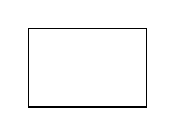
\begin{tikzpicture}[scale=1, baseline=0.2cm]
\draw (0,0)rectangle(1.5,1);
\end{tikzpicture}
}


\parindent=0pt

\title{Activity 2: Generating Keys Using More Realistic Large Integers}
\author{}
\date{}

\begin{document}

\maketitle

In real-life, encryption uses far larger numbers that would be very hard to guess. In Activity 2 we will use more realistic larger numbers.

Drawing up modular tables would take a very long time, so we will use a special mathematical technique, a kind of shortcut for finding modular inverses.

The second `message' will be an integer corresponding to a three-letter word you will select from the table attached.

\section*{Choose Your Keys}

\begin{enumerate}[itemsep=.5cm]
    \item Choose a number $A$ between 25 and 50. \hfill $A = $ \emptybox
    
    \item Choose a second number $B$ between 25 and 50. \hfill $B = $ \emptybox
    
    \item Multiply $A$ and $B$. Call this number $C$. \hfill $C = $ \emptybox
    
    \item Subtract 1. Call this number $D$. \hfill $D = $ \emptybox
\end{enumerate}

\begin{itemize}[itemsep=0.5cm]
    \item Your \textbf{public key} is $A + B + C$ \hfill Public key $= $ \emptybox
    
    \item Your \textbf{encryption key} is $A + D$. \hfill Encryption key $= $ \emptybox
    
    \item Your \textbf{decryption or private key} is $B + D$. \hfill Decryption key $= $ \emptybox
\end{itemize}

\textbf{Tell all others their public and encryption keys. Your decryption key is kept private!}

Now if you took a lot of trouble to check, you would find that:

\begin{center}
\textbf{Encryption key $\times$ Decryption key $= 1$ in the modulus of our Public key.}
\end{center}

We are finally ready to \textbf{encode} and \textbf{decode} our secret message as we have found two numbers whose product is 1 in the modulus of our private key.

\newpage

\section*{Encryption}

Choose a message for transmission from the sheet of three letter words attached.

\begin{enumerate}
    \setcounter{enumi}{4}
    \item Note the number corresponding to your word in the table and multiply it by your \textbf{encryption key}
    
    \[
    F = \text{Message (using table)} \times \text{Encryption key} = \emptybox
    \]
    
    \item Divide $F$ by the \textbf{public key} and write down only those digits appearing in front of the decimal point. \hfill $G = $ \emptybox
    
    \item Multiply $G$ by your \textbf{public key}. \hfill $H = $ \emptybox
    
    \item Subtract $H$ from the result in $F$ above. \hfill $I = $ \emptybox
    
    The result is your encrypted secret word. \hfill \textbf{Encrypted message}
\end{enumerate}

\section*{Decryption}

\begin{enumerate}
    \setcounter{enumi}{8}
    \item Multiply the encoded message in $I$ above by the \textbf{decryption key}. \hfill $J = $ \emptybox
    
    \item Divide the result in $J$ by the \textbf{public key}. Write down only those digits appearing in front of the decimal point. \hfill $K = $ \emptybox
    
    \item Multiply the result in $K$ by the \textbf{public key}. \hfill $L = $ \emptybox
    
    \item Subtract the result in $L$ from the result in $J$. \hfill $M = $ \emptybox
\end{enumerate}

The result is your decrypted message -- a number revealing your secret three-letter word, known only to those who have your private \textbf{decrypting key} alongside your \textbf{public key}.

\newpage

\section*{Table of Three-Letter Words}

\begin{multicols}{6}
\small
\begin{tabular}{cl}
\toprule
\# & Word \\
\midrule
1 & ace \\
2 & act \\
3 & add \\
4 & ado \\
5 & ads \\
6 & adz \\
7 & aft \\
8 & age \\
9 & ago \\
10 & aha \\
11 & aid \\
12 & ail \\
13 & aim \\
14 & air \\
15 & alb \\
16 & ale \\
17 & all \\
18 & amp \\
19 & and \\
20 & ani \\
21 & ant \\
22 & any \\
23 & ape \\
24 & apt \\
25 & arc \\
26 & are \\
27 & ark \\
28 & arm \\
29 & art \\
30 & ash \\
31 & ask \\
32 & asp \\
33 & ate \\
34 & auk \\
35 & awe \\
36 & awl \\
37 & axe \\
38 & aye \\
39 & baa \\
40 & bad \\
41 & bag \\
42 & bah \\
43 & ban \\
44 & bar \\
45 & bat \\
46 & bay \\
47 & bed \\
48 & bee \\
\bottomrule
\end{tabular}

\columnbreak

\begin{tabular}{cl}
\toprule
\# & Word \\
\midrule
49 & beg \\
50 & bet \\
51 & bib \\
52 & bid \\
53 & big \\
54 & bin \\
55 & bit \\
56 & boa \\
57 & bob \\
58 & bog \\
59 & boo \\
60 & bop \\
61 & bow \\
62 & box \\
63 & boy \\
64 & brr \\
65 & bud \\
66 & bug \\
67 & bum \\
68 & bun \\
69 & bur \\
70 & bus \\
71 & but \\
72 & buy \\
73 & bye \\
74 & cab \\
75 & cad \\
76 & cam \\
77 & can \\
78 & cap \\
79 & car \\
80 & cat \\
81 & caw \\
82 & chi \\
83 & cob \\
84 & cod \\
85 & cog \\
86 & con \\
87 & coo \\
88 & cop \\
89 & cot \\
90 & cow \\
91 & cox \\
92 & coy \\
93 & cry \\
94 & cub \\
95 & cud \\
96 & cue \\
\bottomrule
\end{tabular}

\columnbreak

\begin{tabular}{cl}
\toprule
\# & Word \\
\midrule
97 & cup \\
98 & cur \\
99 & cut \\
100 & dab \\
101 & dad \\
102 & dam \\
103 & day \\
104 & deb \\
105 & den \\
106 & dew \\
107 & did \\
108 & die \\
109 & dig \\
110 & dim \\
111 & din \\
112 & dip \\
113 & dis \\
114 & doc \\
115 & doe \\
116 & dog \\
117 & don \\
118 & dos \\
119 & dot \\
120 & dry \\
121 & dub \\
122 & dud \\
123 & due \\
124 & dug \\
125 & duh \\
126 & dun \\
127 & duo \\
128 & dye \\
129 & ear \\
130 & eat \\
131 & ebb \\
132 & eel \\
133 & egg \\
134 & ego \\
135 & eke \\
136 & elf \\
137 & elk \\
138 & ell \\
139 & elm \\
140 & ems \\
141 & emu \\
142 & end \\
143 & eon \\
144 & era \\
\bottomrule
\end{tabular}

\columnbreak

\begin{tabular}{cl}
\toprule
\# & Word \\
\midrule
145 & ere \\
146 & erg \\
147 & err \\
148 & eta \\
149 & eve \\
150 & ewe \\
151 & eye \\
152 & fad \\
153 & fan \\
154 & far \\
155 & fat \\
156 & fax \\
157 & fed \\
158 & fee \\
159 & fen \\
160 & fer \\
161 & few \\
162 & fey \\
163 & fez \\
164 & fib \\
165 & fie \\
166 & fig \\
167 & fin \\
168 & fir \\
169 & fit \\
170 & fix \\
171 & flu \\
172 & fly \\
173 & fob \\
174 & foe \\
175 & fog \\
176 & fop \\
177 & for \\
178 & fox \\
179 & fro \\
180 & fry \\
181 & fun \\
182 & fur \\
183 & gab \\
184 & gad \\
185 & gag \\
186 & gal \\
187 & gap \\
188 & gas \\
189 & gee \\
190 & gel \\
191 & gem \\
192 & get \\
\bottomrule
\end{tabular}

\columnbreak

\begin{tabular}{cl}
\toprule
\# & Word \\
\midrule
193 & gig \\
194 & gin \\
195 & gnu \\
196 & gob \\
197 & god \\
198 & goo \\
199 & gos \\
200 & got \\
201 & gum \\
202 & gun \\
203 & gut \\
204 & guy \\
205 & gym \\
206 & gyp \\
207 & had \\
208 & hag \\
209 & hah \\
210 & ham \\
211 & has \\
212 & hat \\
213 & haw \\
214 & hay \\
215 & hem \\
216 & hen \\
217 & hep \\
218 & her \\
219 & hes \\
220 & hew \\
221 & hex \\
222 & hey \\
223 & hid \\
224 & hie \\
225 & him \\
226 & hip \\
227 & his \\
228 & hit \\
229 & hob \\
230 & hod \\
231 & hoe \\
232 & hog \\
233 & hop \\
234 & hos \\
235 & hot \\
236 & how \\
237 & hub \\
238 & hue \\
239 & hug \\
240 & huh \\
\bottomrule
\end{tabular}

\columnbreak

\begin{tabular}{cl}
\toprule
\# & Word \\
\midrule
241 & hum \\
242 & hut \\
243 & ice \\
244 & icy \\
245 & ids \\
246 & ifs \\
247 & ilk \\
248 & ill \\
249 & imp \\
250 & ink \\
251 & inn \\
252 & ins \\
253 & ion \\
254 & ire \\
255 & irk \\
256 & ism \\
257 & its \\
258 & ivy \\
259 & jab \\
260 & jag \\
261 & jam \\
262 & jar \\
263 & jaw \\
264 & jay \\
265 & jet \\
266 & jib \\
267 & jig \\
268 & job \\
269 & jog \\
270 & jot \\
271 & joy \\
272 & jug \\
273 & jut \\
274 & keg \\
275 & ken \\
276 & key \\
277 & kid \\
278 & kin \\
279 & kit \\
280 & lab \\
281 & lad \\
282 & lag \\
283 & lam \\
284 & lap \\
285 & law \\
286 & lax \\
287 & lay \\
288 & lea \\
\bottomrule
\end{tabular}
\end{multicols}

\vfill

\noindent\small
\textcopyright{} 2016 Education Services Australia Ltd, unless otherwise indicated.\\
Creative Commons BY 4.0 license, unless otherwise indicated.

\end{document}
